\chapter{METODOLOGÍA}

El tipo de investigación realizada es de enfoque experimental, este tipo de investigación consiste en la manipulación directa de una variable independiente, la comparación de dos o mas grupos de condiciones, la medición de cada variable de forma dependiente y un diseño con estadística inferencial que permita el control máximo de variables extrañas.\parencite{MoroneMetodosCientifica}

El proyecto estará dividido en tres fases organizadas y estructuradas para abarcar la totalidad del mismo de forma ágil y efectiva, estas son, fase de análisis, fase de diseño y construcción, y fase de evaluación o validación del producto.

A continuación, se realiza una descripción de cada una de ellas, comenzando en la fase de análisis 
\begin{itemize}
\item Elaboración de entrevistas con profesionales en Salud y seguridad en el trabajo (SST), Salud ocupacional y medicina, como herramienta de investigación se realizará el cuestionario clave para entrevistas a profesionales en el área a SST.
\item Aplicación de entrevistas a profesionales en Salud y seguridad en el trabajo (SST), Salud ocupacional y medicina.
\item Revisión bibliográfica, Se realizará una investigación documental, para condensar el volumen de información relacionada procedente de diferentes fuentes que permitan realizar una comparación de diferentes posturas frente a el tema y sintetizar las ideas en el proyecto. 
\item Consolidación del modelo de valoración de riesgo postural, a partir de la información recolectada de los profesionales y los referentes nacionales e internacionales se realiza un modelo que desde la ergonomía identifique hasta donde un movimiento con cierta repetividad y ángulo se convierte en un riesgo. 
\item Afianzamiento de parámetros de entrada, se definen los posibles parámetros de entrada del sistema.
\item Exploración de técnicas con IA para clasificación, la selección de la herramienta de IA es importante para correcta ejecución del proyecto, por lo tanto, se realizará una exploración de las técnicas posibles que responden al problema de clasificación identificado. 

\end{itemize}

La siguiente fase está denominada como fase de diseño y construcción, la cual está dividida en la siguientes sub-fases.
\begin{itemize}
\item Diseño del modelo arquitectural, Se realiza el diseño arquitectural del prototipo de software, contemplando la estructura entre los elementos y las relaciones de estos.
\item Validación del modelo arquitectural, Es un proceso en el que se validará el nivel de abstracción del modelo y verificación de la correctitud técnica, esto permitirá asegurar la integridad técnica del prototipo a construir.  
\item Diseño modulo preparación de datos (recolección y tratamiento), Se definirá el proceso de organización y normalización de los datos recolectados para tratamiento.
\item Selección de técnica de IA para clasificación, se determinará cual algoritmo de machine learning se ajusta mejor al problema.
\item Diseño de módulo de interpretación, se identificarán las características que tendrá el modelo de IA, incluyendo el ajuste de los parámetros.
\item Construcción de la herramienta, La herramienta está enmarcada en la metodología ágil SCRUM, posteriormente, dependiendo del modelo arquitectural se definirá la lógica de negocio.

\end{itemize}

Para terminar se realizará la fase de validación en la que se realizará un comprobación de la herramienta contra los resultados teóricos, además se realizarán pruebas piloto supervisadas por profesionales en Salud y seguridad en el trabajo (SST), Salud ocupacional y medicina con la finalidad de obtener las respectivas validaciones y afinar el modelo, para culminar, se realizará la compilación de la documentación y entrega.


\subsection{Metodología de software (SCRUM)}
Las metodologías de software ordenan y promueven buenas prácticas en el desarrollo de software de calidad, actualmente se encuentran numerosos modelos y metodologías que se pueden adaptar dependiendo las necesidades del producto final a entregar\parencite{Nohemy2015ESCOGERDECISION}. Para el proyecto ErgoSent se identificaron dos perspectivas importantes que orientan la selección de la metodología, inicialmente debe permitir el desarrollo en un marco de tiempo corto; para este proyecto en específico de 6 meses y por otra parte necesita una verificación diaria con participación constante de expertos, permitiendo un crecimiento preciso y controlado, en donde se tomen decisiones rápidas y adaptables acorde al desarrollo de la aplicación.


Antes de comenzar es necesario definir el producto, el equipo de SCRUM y las tareas generales a realizar, para así elaborar la estructura del proyecto con la metodología, el equipo de trabajo estará compuesto así: 
\begin{itemize}
    \item Product Owner:  Con el objetivo de tener varios puntos de vista, hemos conseguido un grupo de profesionales que nos permiten tener una visión interdisciplinar para cumplirán este rol.
    \begin{enumerate}
        \item Diana Rivera Castillo, Ingeniera industrial con especialización en salud ocupacional, Youtuber Colombiana más influyente en Salud y seguridad en el trabajo SST, y actual Gerente de HSEQ Nueva Visión.
        \item Jorge Enrique Moreno Collazos, Fisioterapeuta, especialista en rehabilitación Cardiopulmonar, magíster en ciencias de la actividad física y el deporte, magíster en calidad educativa, doctor en salud pública, doctor en terapia manual, doctor en educación, Pos doctorado en educación, ciencias sociales e interculturalidad. Docente e investigador.
        \item Ximena Cano, Médica de la Universidad de Ciencias Aplicadas y Ambientales U.D.C.A. 
    \end{enumerate}

\item Scrum Master: esté cargo estará ocupado por Daniel Nieto Gomez.
\item Equipo desarrollador: Estará compuesto por Junior Parra como desarrollador de Scripting en Back end C\# y análisis de software, junto con Daniel Nieto Gómez como diseñador y desarrollador Front end y Análisis enfocado en el uso de herramientas de IA (inteligencia artificial). 
\end{itemize}

La duración del Sprint será de 2 semanas, por el periodo correspondiente al proyecto, es decir, 6 meses.

Por tratarse de un producto de software, la primera tarea a llevar a cabo es la ingeniería o levantamiento de requerimientos, identificando los casos de uso más importantes y requisitos de alto nivel, discutiéndolos con los product owners y  partes interesadas, posteriormente, se escriben en el SCRUM product Backlog y se da inicio a la estimación y priorización de las sesiones con el equipo SCRUM, Luego se comienzan a dividir los requerimientos de alto nivel en requerimientos más pequeños, que se puedan enmarcar en historias de usuario, una vez realizada esta tarea, se convoca a la reunión de planeación del primer Sprint (Sprint planning meetting).

\begin{figure}[H]
    \centering    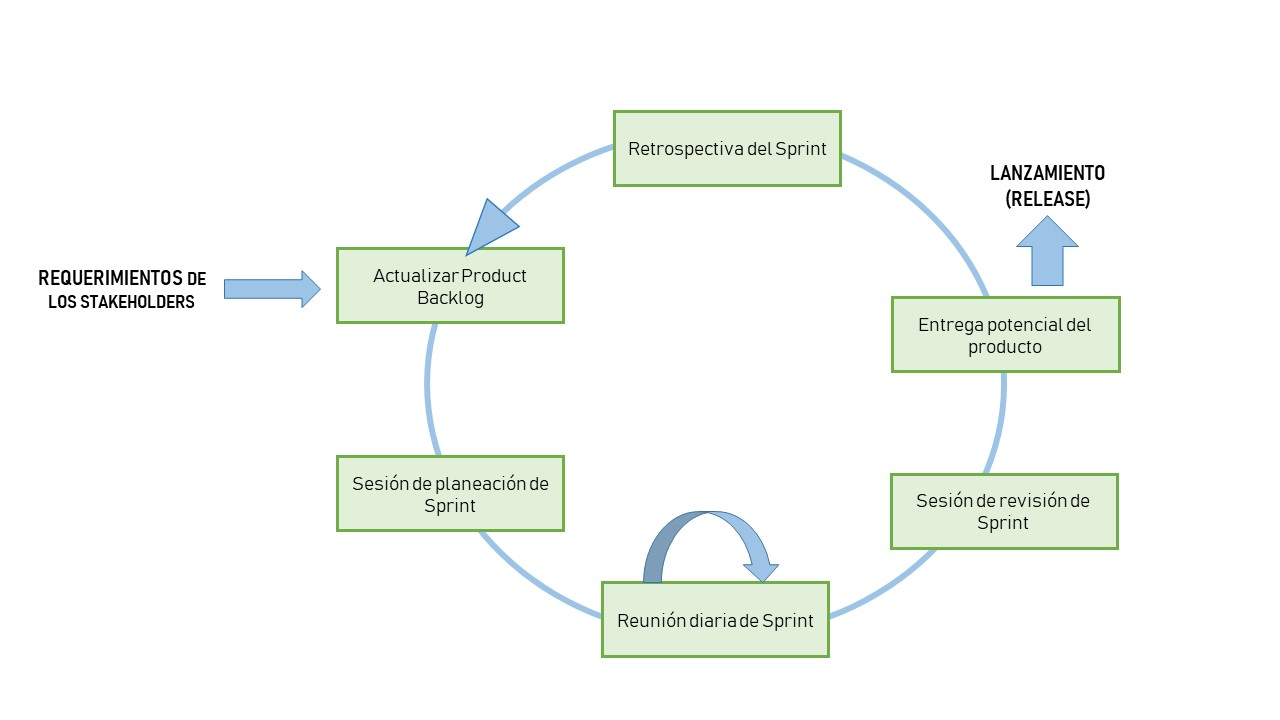
\includegraphics[width=1\textwidth]{Anexos/LATEX/chapters/images/Scrum_1.jpg}
    \caption{Diagrama de Fases y Sprints para el proyecto}
    \small{\textbf{Fuente:} Elaboración propia}
    \label{SCRUM2}
\end{figure}

Con la finalidad de dar soporte a los sprint diarios, se utilizará la plataforma de desarrollo colaborativo Github, facilitando el alojamiento del proyecto y obteniendo control sobre el versionamiento.






